\setstretch{1.5}
\chapter{Protocol}
\section{Introduction}
\subsection{Background}
Idiopathic Parkinson's disease (\acs{iPD})\acused{iPD} represents a chronic neurodegenerative disorder manifested by both motor and non-motor symptoms. The physical impairments in \ac{iPD} have a significant psychosocial impact and lead to considerable losses in patients'  \ac{QoL} and a high burden on (informal) caregivers. Several \ac{QoL} assessment tools have been developed so far, some of which are specific to \ac{iPD} \cite{stuhrenberg2022jpm}. However, none of the models take into account positive aspects of well-being or a subject's personal attitude (e.g., optimism) but also manifold aspects in someone's life such as lack of social support as possible stress factor or level of integration, to name a few. In the present project, an investigation of \ac{iPD}-patients' \ac{QoL} over time will be carried out. For this purpose, a longitudinal assessment using established and validated \ac{HRQOL}-questionnaires will be performed. In addition, holistic observations are intended using the the so-called \textsc{CHAPO}-model -- an approach originally developed for the assessment of life quality of very old people\footnote{\url{https://ceres.uni-koeln.de/forschung/nrw80}}. By adapting it to aspects of \ac{iPD}-patients, the so-called \acs{CHAPO}-\textsc{PD}-model \cite{thieken2022jpd} will be applied in this cohort study. The aim of this project is thus to record \ac{QoL} in a standardised way over a long period of time. This data will be additionally put into context to biomarkers obtained annually in form of a cranial \ac{MRI} and data obtained from blood, saliva, urine, hair and stool samples. We envisage the identification of biomedical markers with predictive value for \ac{QoL} changes. In addition, the approach in this longitudinal study aims at ascertaining the support services needed to better address the needs of family members of \ac{iPD}-patients. Stress experience, changes in sleep patterns and \ac{QoL} losses over the observation period will be included in the analysis of caregivers to identify a surrogate for adequate support.

\subsection{Geographic context}
\ac{iPD} is one of the most common neurological diseases. Estimates put the incidence of the disease in Germany at \SI{84.1}{} per \num[round-precision = 0, round-mode = places]{100000}{} people and per year and assume a number of approx. \num[round-precision = 0, round-mode = places]{400000}{} people \cite{nerius2017parkinson}. In order to understand the special features of the \UKGM as far as the care of \ac{iPD} patients is concerned, it is necessary to know the location of Marburg. Approximately \SI[round-precision = 0, round-mode=places]{77000}{} people live in the city of Marburg which is located in the countryside of the centre of Germany. It is a university town and a district town in the federal state of Hesse (cf. Figure \ref{fig1:hesseGermany}). Due to its location at about \SI{80}{\km} direct distance between the metropolitan areas of Frankfurt am Main and Kassel, the role of the \UKGM must be understood as the predominant centre for medical care in the district. About \num[round-precision = 0, round-mode = places]{1500}{} people with \ac{iPD} are treated there every year. To ensure access to care for patients in the district of Marburg, the \ac{PANAMA} was founded in 2016 by the Neurology Department. In this care network, different actors work together to facilitate the integration of care services and improve outcomes for patients. At the same time, it is a tertiary centre that combines established treatment services for each stage of the disease with university medicine and offers a series of studies that can provide innovative forms of therapy. This makes it possible to offer modern and tailor-made therapy to people from beyond the region.

\begin{wrapfigure}{r}{0.45\textwidth} %this figure will be at the right
    \label{fig1:hesseGermany}
    \centering
    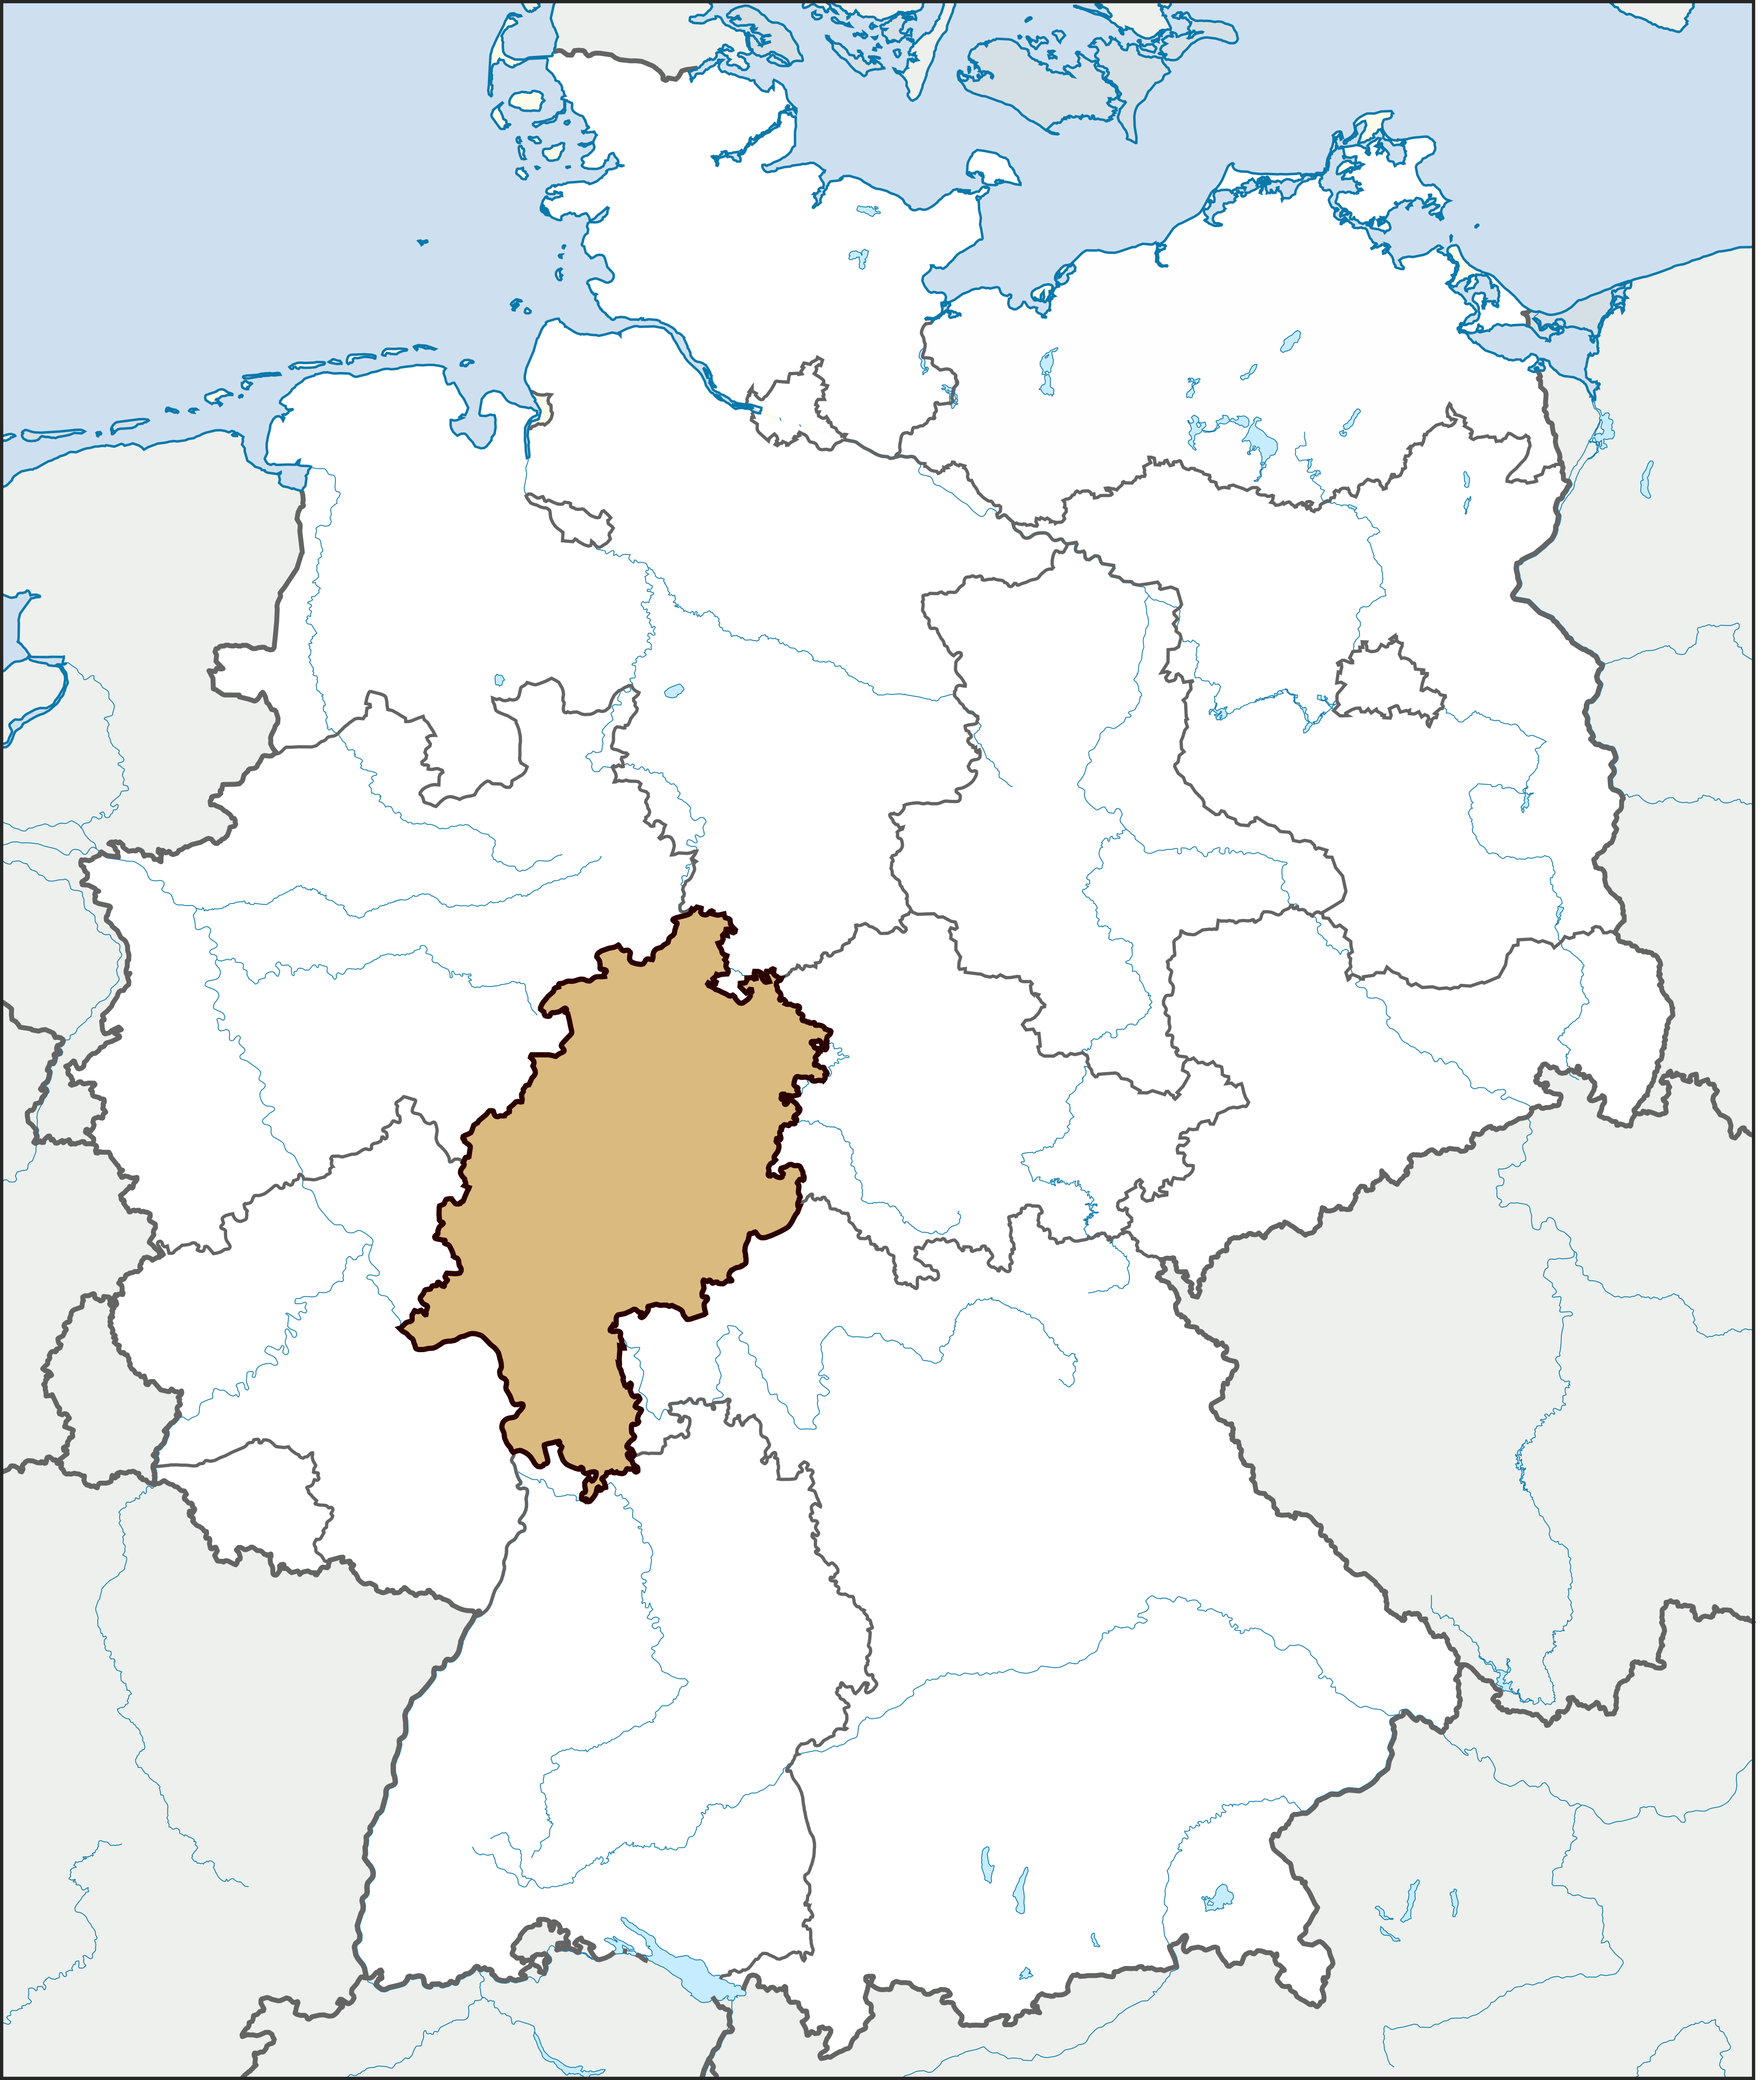
\includegraphics[width=0.45\textwidth]{Hesse_in_Germany.v1.0}
    \caption{Location of Hesse in the German Federal Republic}
\end{wrapfigure}

In order to represent the diversity of the population of \ac{iPD}-patients at \UKGM and to ensure a balanced study cohort, as many of the treated patients as possible should be given the opportunity to participate in the \textsc{HessenKohorte}. Accordingly, the management of the study imposes on itself to adopt the recruitment strategies that have been successfully tested in previous clinical studies and to adapt them to the requirements of the long-term cohort study. To this end, on the one hand, patients are directly offered participation in the study during their appointments in the outpatient clinic of the hospital or during their inpatient stay in the Neurology Department. Secondly, members of \ac{PANAMA} will be made aware of the study with the aim of arousing the interest of potential participants. Finally, detailed information will be made available on the media website of \UKGM to ensure sufficient information (\url{https://www.uni-marburg.de}).
\newpage

%%%%%%%%%%%%%%%%%%%%%%%%%%%%%%%%%%%%%%%%%%%%%%%%%%%%%%%%%%%%%%%%%%%%%%%
%%%% 										START OF SYNOPSIS												%%%%
%%%%%%%%%%%%%%%%%%%%%%%%%%%%%%%%%%%%%%%%%%%%%%%%%%%%%%%%%%%%%%%%%%%%%%%

\setstretch{1}
\section{Protocol synopsis}
\begin{tabularx}{1\textwidth}{m{3.5cm} | X}
\toprule
%\multicolumn{2}{c}{}\\
\multicolumn{2}{p{\dimexpr\linewidth-2\tabcolsep-2\arrayrulewidth}|}
{\textbf{
 Longitudinal digital observation of the holistic quality of the life of patients with \acl{iPD} and their caregivers: a prospective observational cohort study
}}
\\ \toprule

\textbf{Study objectives} & 
This study aims at observing \ac{QoL} of \num[round-precision = 0, round-mode = places]{1000} patients suffering from \ac{iPD} and their relatives over the course of 20 years and relating this to a objectifiable changes in the metabolism but also to structural imaging changes during this time.
\\ \midrule

\textbf{Study design} &
Prospective single-center observational cohort study
\\ \midrule

\textbf{Planned Number of Subjects} &
\num[round-precision = 0, round-mode = places]{1000} 
\\ \midrule

\textbf{Primary Endpoint} &
Quality of life of the index patient after an observation of up to 20 years
\\ \midrule

\textbf{Secondary Endpoints} & 
\tabitem{Index of the \ac{QoL} of the relatives of patients after a follow-up of up to 20 years} \\
& \tabitem{Changes in motor symptoms of the index patient after up to 20 years} \\
& \tabitem{Development of non-motor symptoms over up to 20 years} \\
& \tabitem{Changes of the functional imaging over the observational period} 
\\ \midrule

\textbf{Enrollment of participants} & Patients suffering from \ac{iPD} may be enrolled together with their relatives at any point in time.
\\ \midrule

\textbf{Study visits schedule} & 
\tabitem{Screening} \\
& \tabitem{Baseline Visit}\\
& \tabitem{Yearly follow-up}\\
& \tabitem{\ldots}\\
& \tabitem{Visit at year 2042 (\textit{End-of-Study}-visit)} 
\\ \midrule 

\textbf{Study Duration} &
The study will be considered complete after all subjects complete their visit in the year 2042. Hence, the total study duration is estimated to be at most 20 years.
\\ \midrule

\textbf{Inclusion criteria \ac{iPD}-patients} &
\tabitem{Patients suffering from a clinical diagnosis of \acs{iPD} according to the recent clinical diagnostic criteria \cite{postuma2015mds}} \\
& \tabitem{\ac{iPD}-stages of \RNum{1} -- \RNum{4} according to the Hoehn \& Yahr
  scale (in the OFF state, i.e., without medication) \cite{hoehn1967parkinsonism}} \\
& \tabitem{Patients aged between between 30 and 100 years} \\
& \tabitem{Patients with the ability to provide informed consent. In
  cases where participants lose their capacity to consent at follow-up
  visits (e.g., due to dementia, etc.), this participant will only be
  allowed to continue if a legal representative (proxy, guardian)
  provides informed consent to further participation on behalf of the
  participant. In this case, the legal representatives will be
  provided with a separate consent form.} \\
\\ \midrule

\textbf{Exclusion criteria \ac{iPD}-patients} &
\tabitem{Patients suffering from a clinical diagnosis of atypical 
  Parkinson's syndrome in a first instance. Patients enrolled who
  were later characterized as atypical Parkinson syndroms will not be
  excluded.}\\
& \tabitem{\ac{iPD}-stages of \RNum{5} according to the Hoehn \& Yahr scale
  (in the OFF stage, i.e. without medication) \cite{hoehn1967parkinsonism}}\\
& \tabitem{The use of magnetic fields in the MRI examination excludes
  the participation of persons who have electrical devices
  (e.g., cardiac pacemakers, medication pumps, etc.) or metal parts
  (e.g., screws after bone fracture) in or on their bodies.} \\
& \tabitem{Women who are pregnant will not receive \ac{MRI}.} \\
& \tabitem{Subjects who do not want to be informed about possible
  incidental findings are also not allowed to participate in the
  imaging part of the study.}
\\ \midrule

\textbf{Inclusion criteria \ac{iPD}-patients' relatives} &
\tabitem{Relatives of patients included in the study according to the abovementioned criteria} \\
& \tabitem{Subjects with the ability to give informed consent} \\
\\ \midrule

\textbf{Exclusion criteria \ac{iPD}-patients' relatives} &
Relatives who are unable to give informed consent cannot be considered for study participation
\\ \midrule

\textbf{Statistical methods} &
Due to a large number of possible primary endpoints for consideration, a multitude of analyses will be conducted to examine changes and variability over the 20 years. Analyses will include logistic, linear, and longitudinal models for assessing these data, among others. Primary interest will focus on established and longterm measures of quality-of-life (such as the \ac{PDQ39}\cite{jenkinson1997pdq39}) but also of clinical severity such as the \ac{MDS-UPDRS}\cite{goetz2007updrs}. For the secondary endpoints, clinical, imaging, and biological verification studies, on promising biological markers in study subsets using stored collected samples sould be performed. These studies may vary substantially depending on the type of marker and the data available.
\\ \midrule

\textbf{Statistical test method} & 
According to the primary endpoint and the envisaged number of participants, \ac{ANOVA} will be conducted in order to determine the predictors of decreases in \ac{QoL} during the \ac{iPD}-patients' course. Furthermore, studies correlating \ac{QoL} to the identified markers and results in imaging should be performed. 
\\ \midrule

\textbf{Sample Size Parameters} & 
This is a longitudinal cohort study where the number of participants is determined by the number of resources available. The number of participants is therefore composed of the expected number of patients in the district and the resources available to the centre (\UKGM).
\\ \bottomrule
\end{tabularx}
\newpage

%%%%%%%%%%%%%%%%%%%%%%%%%%%%%%%%%%%%%%%%%%%%%%%%%%%%%%%%%%%%%%%%%%%%%%%
%%%% 										END OF SYNOPSIS													%%%%
%%%%%%%%%%%%%%%%%%%%%%%%%%%%%%%%%%%%%%%%%%%%%%%%%%%%%%%%%%%%%%%%%%%%%%%

\setstretch{1.5}
\section{Study objectives and endpoints}
\subsection{Study objectives}
The primary aim of the \textsc{HessenKohorte} is to deepen the understanding of the development of \ac{QoL} in \ac{iPD}-patients and to identify factors with favourable or detrimental impact thereon in an average German cohort. Furthermore, the study aims at improving our understanding of the diseases' impact on the caregivers and to find out which factors or forms of structural support make these family caregivers more resilient to those burdens resulting while caring for a person with \ac{iPD}.

\subsection{Primary study endpoint}
The primary endpoint of the \textsc{HessenKohorte} is the index patients' \ac{QoL}. For that, a model was developed which measures not only the disease related aspects of life quality (\ac{CHAPO-PD}) but also additional factors which foster \ac{QoL} and thus go beyond healthcare-related issues. This will be ascertained along with established questionnaires such as the \ac{PDQ39}\cite{jenkinson1997pdq39}, or the \ac{WHOQoL}\cite{group1998world} and may be related to other characteristics of included patients.

\subsection{Secondary study endpoint}
According to the large number of possible analyses and secondary endpoints for consideration, the authors foresee a substantial
number of analyses to be conducted in order to contemplate changes over time. Yet, a list of a few possible secondary endpoints should be named:
\begin{itemize}
  \item{Changes in motor symptoms of the index patient after up to 20 years}
  \item{Development of non-motor symptoms over up to 20 years}
  \item{Changes of the structural imaging over the observational period} 
\end{itemize}
Irrespective of the unique characteristics of a study on \ac{QoL} of people with \ac{iPD}, standard examinations of \ac{iPD}-patients should also be carried out as far as the secondary endpoints are concerned. At this point, motor along with non-motor symptoms should be mentioned as the most common symptoms encountered. The former constitute the hallmark of the disease, whereas the latter are incresingly recognized as responsible for huge losses in \ac{QoL} (Quelle). The extent of motor symptoms will be operationalised via part III of the \ac{MDS-UPDRS}\cite{goetz2007updrs}. Non-motor symptoms will be measured using the \ac{NMSQ} a measure able to capture a wide variety of different aspects with regard to this symptom domain. A table with all questionnaires can be found at ()

% Please add a table with all questionnaires @Urs

\section{Study design}
The \textsc{HessenKohorte} is a longitudinal, observational, natural history study to assess \ac{QoL} progression in study participants suffering from \ac{iPD}. The intended cohort size of \num[round-precision = 0, round-mode = places]{1000}{} will be comprehensively assessed for a maximum of five years. All subjects along with their relatives will undergo clinical assessments (motor, non-motor, cognitive neuropsychiatric and \ac{QoL}) and imaging assessments, and will be asked to donate biosamples including blood, urine, saliva, hair and stool. Participants will also be asked to respond to questionnaires and provide digital data as part of the \textsc{HessenKohorte}.

\subsection{Scale and duration}
The study will accompany up to \num[round-precision = 0, round-mode = places]{1000}{} patients over at most 20 years to enable a profound insight into the course of patients' and relatives' \ac{QoL}.

\subsection{Justification for study design}
The \textsc{HessenKohorte} is a single-centre, longitudinal and observational follow-up assessment of \ac{iPD}-patients' \ac{QoL}. This unique primary endpoint will be assessed using a newly developed questionnaire, the main feature of which is a holistic assessment that looks not only at disease-related limitations but also at existing resources and the social environment of those affected \cite{thieken2022jpd}. Accordingly, the inclusion of relatives is fundamental to obtain effects of the disease on the patient's entire environment. The comparatively large number of subjects should provide a good insight into the lives of \ac{iPD}-patients with their multi-layered phenotypes, but also offer possibilities for diverse investigations through the additional recording of biosamples.

\subsection{Hypotheses}
\label{sec:hypoTheses}
The primary endpoint of the study is the development of \ac{iPD}-patients' \ac{QoL} over the course of up to 20 years. The \textsc{HessenKohorte} thereby addresses the following main scientific hypothesis:
\begin{itemize}
  \item Exploratory analysis of the development of \acl{QoL} over the course of the disease.
\end{itemize}
The design of the study is based on the currently accepted assumption that \ac{QoL} of \ac{iPD}-patients correlates significantly with the symptom severity. It can also be assumed that the \ac{QoL} of those affected strongly relates to that of their relatives. The present study design is intended to contribute to its longitudinal assessment, but especially to allow exploratory studies in the course of or at the end of data collection, which could provide information on whether certain factors in the behavioural data, the imaging or the biospecimens provided could have a predictive value.

\subsection{Planned analyses}
Our main method for assessing our hypotheses are linear regression and correlation analyses. In particular we will analyse the correlation between the \ac{QoL} of the index patient and of her relatives and caregivers. In order to extend this analysis we will assess different influencing factors as e.g. age, gender, symptom burden (motor and non-motor). Furthermore in an attempt to elucidate the causal form of the interdependence we will analyse how \ac{QoL} of patients/caregivers at earlier timepoints relates to \ac{QoL} of caregivers/patients at a later point in time.

With regard to our hypothesis concerning the prediction of disease progress, we will primarily rely on linear regression methods. We will try to offer models predicting disease symptoms at the end of the study compared to the status at earlier timepoints. While we first will look at a linear relationship we will also consider more complicated models when they are necessary to model disease progress convincingly. Also in this analysis mediating or moderating variables especially from sociodemographic data may play a role and will accordingly be considered.

\begin{figure}[h]
\label{fig2:scheme}
\centering
\includegraphics[width=1\textwidth]{Schema_HessenKohorte.v1.0}
\caption{Schematic overview of the planned analyses. Subjects will be enrolled subsequently and will receive regular follow-ups. In addition to clinical data in form of different questionnaires, biomarkers including cranial \ac{MRI}, blood, saliva, urine, hair and stool samples will be collected at an annual basis.}
\end{figure}


\section{Subject selection}
\label{sec:study_selection}
\subsection{Study population and Eligibility}
\label{sec:study_population}
Study candidates will be drawn from the patients treated in the Neurology Department of the \UKGM, Marburg site, as either in- or outpatients. Moreover, patients suffering from \ac{iPD} may submit a request for participation in the study. The inclusion and exclusion criteria (cf. Section \ref{sec:inclusion_criteriaIPS}) are checked by one of the study physicians, who are responsible for the final decision. Advertising for the study can be found in the form of a flyer, which is available in the Department of Neurology, but also in the form of an internet homepage, where the project will be presented to the public.

\subsection{Inclusion and exclusion criteria \ac{iPD}-patients}
\label{sec:inclusion_criteriaIPS}
Subjects who meet all the following inclusion criteria may be given consideration for inclusion in this cohort study, provided no exclusion criteria are met (for both, cf. table \ref{tab:inclusionexclusionCriteriaPatients}).

\begin{tabularx}{\textwidth}[!h]{X|X}
\caption{Inclusion and exclusion criteria for \ac{iPD}-patients to participate in the \textsc{HessenKohorte}}\label{tab:inclusionexclusionCriteriaPatients}\\
\toprule
\tabitem{Patients suffering from a clinical diagnosis of \ac{iPD} according to the recent clinical diagnostic criteria \cite{postuma2015mds}} & \tabitem{Patients suffering from a clinical diagnosis of atypical Parkinson's syndrome in a first instance. Patients enrolled who were later characterized as atypical Parkinson syndroms will not be excluded.} \\
\tabitem{\ac{iPD}-stages of I - IV according to the Hoehn \& Yahr scale\cite{hoehn1967parkinsonism} (in the OFF stage, i.e., without medication)} & \tabitem{\ac{iPD}-stages of V according to the Hoehn \& Yahr scale \cite{hoehn1967parkinsonism} (in the OFF stage, i.e. without medication)} \\
\tabitem{Patients with the ability to provide informed consent. In cases where participants lose this capacity at follow-up visits (e.g., due to dementia, etc.), participants will only be allowed to continue if legal representative provides informed consent to further participation on hisor her behalf. In this case, the legal representative will be provided with a separate consent form \ref{einfügen}} & \tabitem{The use of magnetic fields in the \ac{MRI} examination excludes the participation of persons who have electrical devices (e.g., cardiac pacemakers, medication pumps, etc.) or metal parts (e.g. screws after bone fracture) in or on their bodies.}\\
& \tabitem{Women who are pregnant will not receive \ac{MRI} scans.} \\
& \tabitem{Subjects who do not want to be informed about possible incidental findings are also not allowed to participate in the imaging part of the study.} \\
\bottomrule
\end{tabularx}
% TODO: Can we make the bulletpoint „independent“? That is, is it possible to avoid blank spaces just because the other side of the table has a longer bullet point? 

\subsection{Inclusion criteria \ac{iPD}-patients' relatives}
\label{sec:inclusion_criteriaREL}
Only if a patient is included, the relatives may be asked for participation in the study. Subjects who agree to take part in the \textsc{HessenKohorte} must meet all the following inclusion and exclusion criteria (cf. Table  \ref{tab:inclusionexclusionCriteriaRelatives}).


\begin{tabularx}{\textwidth}{X | X}
\caption{Inclusion and exclusion criteria for relatives of \ac{iPD}-patients to participate in the \textsc{HessenKohorte}}\label{tab:inclusionexclusionCriteriaRelatives}\\
\toprule
\tabitem{Relatives of \ac{iPD}-patients included in the study according to the abovementioned criteria (cf. Table \ref{tab:inclusion_exclusionCriteriaPatients})} & \tabitem{Relatives who are unable to give informed consent} \\
\tabitem{Relatives with the ability to give informed consent} &  \\
& \\ 
\bottomrule
\end{tabularx}

\section{Subject accountability}
\subsection{Point of enrollment}
Subject will be considered enrolled at the time of the study-specific \ac{ICF} execution. No study-related procedures or assessments can take place until the \ac{ICF} is signed.

\subsection{Withdrawal}
All enrolled subjects (including those who have dropped out) must be recorded and documented. In case participants drop out of the study, an end-of-study form (\ref{sec:EOSform}) must be filled out and asked for the reasons for dropping out. 

Reasons for withdrawal include but are not limited to:
\begin{itemize}
  \item subject or relative choice to withdraw consent
  \item lost to follow-up
  \item pregnancy\footnote{\label{note1} only MR-imaging will be discontinued during pregnancy or from the moment of an implantation onwards.}
  \item implantation of electrical devices or metal parts in or on the body\footref{note1}
\end{itemize}

Subjects may withdraw at any time, with or without reason, and without prejudice to further treatment. Applicable \ac{CRF} up to the point of subject withdrawal and an end-of-study form \ref{chap:appendix} must be completed. Any subject deemed lost to follow-up should have a minimum of three documented attempts to contact him/her prior to completion of the end-of-study form. Additional study data may no longer be collected after the point at which a subject has been withdrawn from the study or withdraws consent, for whatever reason. Data collected up to the point of subject withdrawal may be used. Subjects withdrawn after completing the implant procedure will not be replaced 
%TODO: We need to draw and End-of-Study-Form @Urs

\subsection{Lost to follow-up}
Patients who do not react to the invitation to fill ou the questionnaires will be contacted in total three times per mail or email:
\begin{itemize}
\item 30 days before the planned visit
\item at the date of the visit and
\item 30 days thereafter
\end{itemize}
 If there is no answer to this third time, patients will be contacted per telefone in order to find out if there is a problem. Patients who cannot be contacted will receive the same number of mails/calls one year and two years after. In case of three years without response, an end-of-study form (cf. \ref{}) will be filled out and the subject is excluded. Vacant places due to excluded subjects may be filled up 5 and 10 years after the onset of the study.

\subsection{Subject status and classification}
A subject will be considered enrolled in this study at the time of the study-specific \ac{ICF} execution.

\subsection{Enrolment control}
The overall enrollment in the study will be capped at \num[round-precision = 0, round-mode = places]{1000} participants.

\subsection{End-of-study definition}
The study is considered complete when 20 years from the first enrolment are over, in the year 2042.

\section{Study methods}
\subsection{Data collection}
The data collection schedule is shown in Table \ref{}
\newpage
\begin{landscape}
\begin{tabularx}{1\textwidth}{@{}X *{6}{C}@{}}
\caption{Data collection schedule for \ac{iPD}-patients enrolled in the \textsc{HessenKohorte}}\label{tab:DataCollectionPatients}\\
\toprule
\textbf{Visit} 				& \textbf{Screening} 			& \textbf{Baseline visit} 	& \textbf{Year 1,2,3,4, ... , 20 Visit}	& \textbf{Half-year visits in between}  & \textbf{Unscheduled Visit} 	\\
\cmidrule{2-6}
Informed Consent Process 	& $\times$ 					&  						& $\times$\textsuperscript{a} 		& $\times$\textsuperscript{a}		& 							\\
Eligibility criteria			& \multicolumn{2}{c}{$\times$}							& 								& 								& 							\\
Subject demographics 		& \multicolumn{2}{c}{$\times$}							& $\times$\textsuperscript{b}		& $\times$\textsuperscript{b} 		& 							\\
\ac{MDS-UPDRS} 			& \multicolumn{2}{c}{$\times$}							& $\times$ 						& 								& $\times$\textsuperscript{a}	\\
\ac{NMSQ}				& \multicolumn{2}{c}{$\times$}							& $\times$						& $\times$						&							\\
\ac{CHAPO-PD}			& \multicolumn{2}{c}{$\times$}							& $\times$						& $\times$						&							\\
Bloodsample				& \multicolumn{2}{c}{$\times$}							& $\times$						& 								&							\\
Urine sample				& \multicolumn{2}{c}{$\times$}							& $\times$						& 								&							\\
Saliva sample				& \multicolumn{2}{c}{$\times$}							& $\times$						& 								&							\\
Hair  sample				& \multicolumn{2}{c}{$\times$}							& $\times$						& 								&							\\
Stool sample				& \multicolumn{2}{c}{$\times$}							& $\times$						& 								&							\\
\bottomrule
\multicolumn{6}{l}{\footnotesize{\textsuperscript{a}Must be obtained again, in case there is a legal representative}} \\
\multicolumn{6}{l}{\footnotesize{\textsuperscript{b}All subjects will be asked to disclose possible changes}} \\
\multicolumn{6}{l}{\footnotesize{\textsuperscript{c}may be ascertained and entered into database}} \\
\end{tabularx}
\end{landscape}
%TODO: Table is not filling out entire page. Also, horizontal lines would be helpful, as this may be used as a checklist later. @Urs

\newpage

\begin{tabularx}{1\textwidth}[H]{@{}X *{6}{C}@{}}\label{tab:DataCollectionRelatives}\\
\caption{Data Collection Schedule for patients' relatives enrolled in the \textsc{HessenKohorte}}\\
\toprule
\textbf{Visit} 				& \textbf{Screening} 			& \textbf{Baseline visit} 	& \textbf{Year 1,2,3,4,5, ... , 20 Visit} 	& \textbf{Half-year visit in between}	& \textbf{Unscheduled Visit} 	\\
\cmidrule{2-6}
Informed Consent Process 	& $\times$ 					&  						&  								& 								& 							\\
Eligibility criteria			& \multicolumn{2}{c}{$\times$}							& 								& 								& 							\\
Subject demographics 		& \multicolumn{2}{c}{$\times$}							& $\times$\textsuperscript{a}		& $\times$\textsuperscript{a} 		& 							\\
Questionnaire X			& 													& $\times$						& $\times$						& $\times$\textsuperscript{b} 	\\
\bottomrule
\multicolumn{6}{l}{\footnotesize{\textsuperscript{a}All subjects will be asked to disclose possible changes}} \\
\multicolumn{6}{l}{\footnotesize{\textsuperscript{b}may be ascertained and entered into database}} \\
\end{tabularx}
%\end{landscape}

%TODO: This Table is neither filling out entire page. Again, horizontal lines would be helpful, as this may be used as a checklist later. @Urs

\subsection{Candidate screening}
\label{subsec:screening}
Subjects will be screened for participation in the study based on study inclusion and exclusion criteria as listed in Section \ref{sec:study_selection}. Subjects who have provided informed consent and who have been determined to not meet all eligibility requirements will not be considered.

\subsection{Informed consent}
Written informed consent must be obtained from potential study candidates and enrollment is only valid, after subjects sign and date the \ac{ICF} (cf. Section ??).
%TODO: Please add the ICF in the Appendix and add a reference. @Urs
\begin{itemize}
\item Subjects will be asked to sign the \ac{ICF} before study-specific tests or procedures are performed.
\item The idea of the study must be explained, and subjects must be given the time and opportunity to ask questions and have those questions answered to their satisfaction.
\item The \ac{ICF} is study specific and has been approved by the ethics commitee.
\item Written informed consent must be recorded appropriately by means of the subject’s dated signature.
\end{itemize}

\subsection{Questionnaires}
\label{subsec:questionnaires}
\subsubsection{\acl{CHAPO-PD}}
The backbone of the study will be the investigation of QoL. Recent debates suggest that established measurement tools do not capture QoL with a holistic view but focus on the health-related experience of QoL [https://doi.org/10.3390/jpm12050804; https://doi.org/10.1007/s40273-016-0389-9]. Furthermore, it is unclear to date what determinants influence QoL beyond mere disease in PD. It is also unclear how QoL develops over the course of the disease. The HessenKohorte offers a unique opportunity to capture changes in QoL in a large study population and develop a comprehensive understanding of this important concept. The study therefore pursues two goals: (i) the development and validation of a holistic measurement instrument for the assessment of QoL and (ii) the longitudinal observation of health-related quality of life using established measurement instruments (cf. Table 1). 
To fulfil the first goal, an instrument will be developed in the first year of the cohort in an evidence-based, patient-oriented and participatory manner, which will be validated alongside the cohort from the second year onwards.  This means that in addition to a systematic review of existing studies, PwPD will be interviewed about their personal experience of QoL and actively involved in the development process of the instrument according to the INVOLVE-guideline [https://www.invo.org.uk/wp-content/uploads/2019/04/Copro_Guidance_Feb19.pdf]. In this process, the study team is guided by the work from the NRW80+ study in which the experience of QoL of elderly people was investigated for the first time in Germany [https://doi.org/10.1007/s00391-017-1217-3].

\subsubsection{\acl{MDS-UPDRS}}
The \ac{MDS-UPDRS} \cite{goetz2007updrs} evaluates various aspects of \ac{iPD}-patients, including non-motor and motor symptoms. It consists of four parts:
\begin{itemize}
\item Part I: Experiences of daily living (non-motor symptoms), including 13 items.
\begin{itemize}
\item A: Behavioral problems of the patient, as evaluated by the examiner.
\item B: Part on non-motor symptoms completed by the patient, with the assistance of a caregiver if necessary, but independent of the investigator.
\end{itemize}
\item Part II: Experiences of daily living (motor aspects) with 13 items. This part is also a self-report questionnaire to be completed by the patient, with the assistance of a caregiver if necessary, but independent of the investigator.
\item Part III: Motor examination with 18 items. All instructions are read to the patient by the examiner or demonstrated directly, so that this part is completed by the examiner.
\item Part IV: Motor Complications with 6 items. This part contains instructions for the examiner and also instructions to be read to the patient. It combines patient-related information with clinical observations and assessments by the examiner.
\end{itemize}

\subsubsection{\acl{MoCa} (\acs{MoCa})}
The \acl{MoCa} evaluates the performance in different cognitive domains using 16 items. The 30 questions test cognitive abilities such as memory, language production , contextual thinking, attention and concentration, behavior, arithmetic, temporal and spatial orientation, and the ability to recognize complex shapes and patterns. Scores result from the correct completion of the tasks, whereby the cognitive performance in the individual domains but also as an overall score can be quantified. The \ac{MoCa} was developed in 2005 \cite{nasreddine2005moca} and has been used in clinical practice since then. The test must be administered by an examiner, who is separately trained and an assessment sheet, a pen and stopwatch are needed. The duration is about 10 minutes.

\underline{Psychometrics:}
\begin{tabularx}{1\textwidth}[H]{| >{\raggedright\arraybackslash}X | >{\raggedright\arraybackslash}X | >{\raggedright\arraybackslash}X | }
\caption{Psychometrics for the \acl{MoCa}}\\
\hline
 											& Value																					& Source										\\
 \hline
 \textbf{Standard error of measurement (SEM)} 	& 																						& 											\\
 \hline
 \textbf{Minimal clinical difference} 				& 																						& 											\\
 \hline
 \textbf{Normative data} 						& \tabitem{\num{26.2} $\pm$ \num{2.9} } 														& \cite{hoops2009moca}, \cite{thomann2018moca} 		\\
 											& \tabitem{\num{26.1} $\pm$ \num{2.5} German subjects} 										& \cite{nasreddine2005moca} 					\\
 \hline
 \textbf{Internal consistency} 					& Cronbach's $\alpha$ = \num{.83} 															& \cite{nasreddine2005moca}						\\
 \hline
 \textbf{Construct validity} 						& Poor correlation with premorbid IQ (r = \num{.19}, p < \num{.05})								& \cite{dalrymple2010moca}						\\
 \hline
 \textbf{Test/retest reliability} 					& Excellent intraclass correlation (ICC) of \num{.79}, Correlation Coefficient = \num{.92}, p < \num{.001}	& \cite{gill2008moca}, \cite{nasreddine2005moca}		\\
 \hline
 \textbf{Interrater validity/reliability} 				& Excellent intraclass correlation (ICC) of \num{.81}												& \cite{gill2008moca},								\\
 \hline
\end{tabularx}


\subsubsection{\acl{NMSQ}, (\acs{NMSQ})}
The \ac{NMSQ} is a 30-item rater-based scale designed to assess a broad spectrum of non-motor symptoms in patients with \ac{iPD}.
The \ac{NMSQ} measures the severity and frequency of non-motor symptoms across nine dimensions (??).
%TODO: More information is needed on what the domains are and what to consider, etc.

\subsubsection{\acl{BDI} (\acs{BDI})}
The \acl{BDI} measures the severity of depressive symptoms. It consists of 21 items  measuring symptoms on a scale from 0--3. The questionnaire was first introduced in 1991 \cite{beck1987bdi1} and revised to the current version in 1996 \cite{beck1996bdi2}. The self-administered test takes 5--10 minutes to be completed but does not require any special training. Answers are added for the total score, so that results range in a scale of 0--63 points. Higher scores thereby correspond to more severe symptoms. Since its development, the \ac{BDI} has been used to quantify depressive symptoms in non-specific populations, but particularly in patients with stroke, spinal cord injury and \ac{iPD}. 

\underline{Scores:}
\begin{itemize}\itemsep2pt
\item 0--12: no depressive symptoms or clinically inapparent
\item 13--19: mild depressive syndrome
\item 20--28: moderate depressive syndrome
\item $>$ 29 severe depressive syndrome
\end{itemize}

\underline{Psychometrics:}
\begin{tabularx}{1\textwidth}[H]{| >{\raggedright\arraybackslash}X | >{\raggedright\arraybackslash}X | >{\raggedright\arraybackslash}X | }
\caption{Psychometrics for the \acl{BDI}}\\
\hline
											& Value											& Source		\\
\hline
\textbf{Standard error of measurement (SEM)} 	& 												& 		\\
\hline
\textbf{Minimal clinical difference} 				& 												& 		\\
\hline
\textbf{Normative data} 						& 												& 		\\
\hline
\textbf{Internal consistency} 					& \tabitem{Excellent for \ac{iPD}-patients, Cronbach's $\alpha$ = \num{.88}} 		& \cite{levin1988bdi}		\\
											& \tabitem{Excellent for non-specific populations, Cronbach's $\alpha$ = \num{.81}} 		& Beck and Steer 1998 		\\
\hline
\textbf{Construct validity} 						& \numrange{.48}{.79} in psychiatric outpatients 		& \cite{beck1987bdi1}, \cite{beck1996bdi2}, \cite{snyder2000bdi} \\
\hline
\textbf{Test/retest reliability} 					& Excellent intraclass correlation (ICC) of \num{.88} in \ac{iPD}-patients		& \cite{visser2006bdi} \cite{richter1998bdi}		\\
\hline
\textbf{Interrater validity/reliability} 				& 		& 		\\
\hline
\end{tabularx}

\subsubsection{\acl{CBI} (\acs{CBI})}
The \acl{CBI} assesses the presence or severity of symptoms indicative of burnout. In the short version used, the questionnaire consists of 19 items that scale levels of physical and psychological exhaustion in relation to personal, work and client burnout. The CBI was introduced in 2005 by Kristensen et al. \cite{kristensen2005cbi} and is self-administered without special training. It takes about 5-10 minutes to complete. The scale ranges from 1 (``never/very seldom'' or ``to a very low degree'') to 5 (``very often'' or ``to a very high degree''), resulting in a total score of 19--95 by adding the individual scores or individual scales for personal burnout (6--30), work-related burnout (7---36) and client-related burnout (6--30). A higher score indicates higher levels of stress and an increased likelihood of burnout.

\underline{Psychometrics:}
\begin{tabularx}{1\textwidth}[H]{| >{\raggedright\arraybackslash}X | >{\raggedright\arraybackslash}X | >{\raggedright\arraybackslash}X | }
\caption{Psychometrics for the \acl{CBI}}\\
\hline
											& Value											& Source		\\
\hline
\textbf{Standard error of measurement (SEM)} 	& 												& 												\\
\hline
\textbf{Minimal clinical difference} 				& 												& 												\\
\hline
\textbf{Normative data} 						&  \tabitem{Personal burnout: \num{35.9}}				& \cite{kristensen2005cbi}							\\
											&  \tabitem{Work-related burnout: \num{33.0}}			& 												\\
											&  \tabitem{Client-related burnout: \num{30.9}}		& 												\\
\hline
\textbf{Internal consistency} 					&												& 												\\
\hline
\textbf{Construct validity} 						& 												& 												\\
\hline
\textbf{Test/retest reliability} 					& 												& 												\\
\hline
\textbf{Interrater validity/reliability} 				& 												& 												\\
\hline
\end{tabularx}

\subsubsection{\acl{CISS} (\acs{CISS})}
The ``Coping Inventory for Stressful Situations'' (\acs{CISS}) assesses habitual coping with stress in the context of task-oriented coping, emotion-oriented coping and avoidance-oriented coping with a total of 24 and 48 questions respectively. The CISS was originally introduced in 1990 \cite{endler1990ciss} and revised in 2020 for a shortened, German-language version \cite{kalin2020ciss}. The questionnaire is self-administered without special training and takes 10--15 minutes to complete.

%TODO: add further details to how the score is determined, @David?

\underline{Psychometrics:}
\begin{tabularx}{1\textwidth}[H]{| >{\raggedright\arraybackslash}X | >{\raggedright\arraybackslash}X | >{\raggedright\arraybackslash}X | }
\caption{Psychometrics for the \acl{CISS}}\\
\hline
											& Value											& Source		\\
\hline
\textbf{Standard error of measurement (SEM)} 	& 												& 												\\
\hline
\textbf{Minimal clinical difference} 				& 												& 												\\
\hline
\textbf{Normative data} 						&  												& 			\\

\hline
\textbf{Internal consistency} 					&	Task-oriented coping: Cronbach's $\alpha$ = \num{.83} & \cite{kalin2020ciss}	\\
											&	Emotion-oriented coping: Cronbach's $\alpha$ = \num{.80} & \cite{kalin2020ciss} 	\\
											&	Avoidance-oriented coping: Cronbach's $\alpha$ = \num{.79} & \cite{kalin2020ciss}	\\

\hline
\textbf{Construct validity} 						&												& 				\\
\hline
\textbf{Test/retest reliability} 					&												& 				\\

\hline
\textbf{Interrater validity/reliability} 				& 												& 				\\
\hline
\end{tabularx}



\subsubsection{\acl{MFI-20}}
The ``Multidimensional Fatique Inventory – 20'' (\acs{MFI-20}) measures 5 dimensions of fatigue with 20 questions: general fatigue, physical fatigue, reduced activity, reduced motivation and mental fatigue. The \acs{MFI-20} was introduced in 1995 \cite{smets1995mfi20}. It is a self-administered test that requires no special training and is reported to take 5--10 minutes to complete. It includes response options to various fatigue-related statements ranging from ``Yes, this is true'' to ``No, this is not true'', scaled from 1 -- 5 per question, with 4 -- 20 points for each dimension. A high total score on the different dimensions corresponds to a higher level of fatigue in the corresponding dimension.

\underline{Psychometrics:}
\begin{tabularx}{1\textwidth}[H]{| >{\raggedright\arraybackslash}X | >{\raggedright\arraybackslash}X | >{\raggedright\arraybackslash}X | }
\caption{Psychometrics for the \acl{MFI-20}}\\
\hline
											& Value											& Source		\\
\hline
\textbf{Standard error of measurement (SEM)} 	& 												& 												\\
\hline
\textbf{Minimal clinical difference} 				& 												& 												\\
\hline
\textbf{Normative data} 						&  cf. \cite{smets1995mfi20} for chronic fatigued patients, radiotherapy patients, soldiers (in training), physicians, psychology students, medical students															& \cite{smets1995mfi20}										\\

\hline
\textbf{Internal consistency} 					&	General fatigue -- Cronbach's $\alpha$ = \num{.83} -- \num{.90}*			& \cite{smets1995mfi20}	\\
											&	Physical fatigue -- Cronbach's $\alpha$ = \num{.85} -- \num{.93}*			& \cite{smets1995mfi20}	\\
											&	Reduced activity -- Cronbach's $\alpha$ = \num{.53} -- \num{.86}*			& \cite{smets1995mfi20}	\\
											&	Reduced motivation -- Cronbach's $\alpha$ = \num{.57} -- \num{.82}*			& \cite{smets1995mfi20}	\\
											&	Mental fatigue -- Cronbach's $\alpha$ = \num{.77} -- \num{.93}*			& \cite{smets1995mfi20} \\

\hline
\textbf{Construct validity} 						&	Significant differences p<\num{0.001} 				& \cite{smets1995mfi20} \\
\hline
\textbf{Test/retest reliability} 					& 	Cronbach's $\alpha$ $>$ \num{.88}					& \cite{hinz2020mfi20} \\

\hline
\textbf{Interrater validity/reliability} 				& 													&		\\
\hline
Determined in five different populations (radiotherapy patients, chronic fatigued patients, psychology students, medical students and army recruits)											&	& 		\\
% @Urs, please add a footnote or merge the columns to one.
\end{tabularx}


\subsubsection{\acl{PDCB} (\acs{PDCB})}
The `Parkinson's Disease Caregiver Burden Questionnaire''  (\acs{PDCB}) measures level of burden experienced in caring for a person with \ac{iPD}. It consists of 20 questions in 8 domains that indicate the occurrence of various emotional, health and social consequences of caring for persons with \ac{PD}, using a 0--4 point scale by disagreeing (``I disagree'') and gradually increasing agreement (``I strongly agree'') with statements about one's burden. The (\acs{PDCB}) was first introduced in 2013 \cite{zhong2013pdcb}, and revised in 2019 with a German translation \cite{klietz2019pdcb}. It takes 5 -- 10 minutes to be completed and is a self-administered test that requires no special training. The total score of the questionnaire is obtained by adding the individual scores between 0 -- 4 of all 20 questions. A higher score corresponds to a greater burden of caring for a person with \ac{PD}.

\underline{Psychometrics:}
\begin{tabularx}{1\textwidth}[H]{| >{\raggedright\arraybackslash}X | >{\raggedright\arraybackslash}X | >{\raggedright\arraybackslash}X | }
\caption{Psychometrics for the \acl{PDCB}}\\
\hline
											& Value											& Source		\\
\hline
\textbf{Standard error of measurement (SEM)} 	& 												& 												\\
\hline
\textbf{Minimal clinical difference} 				& 												& 												\\
\hline
\textbf{Normative data} 						&  												& 			\\

\hline
\textbf{Internal consistency} 					&												& 												\\
\hline
\textbf{Construct validity} 						&	Cronbach's $\alpha$ = \num{.856}				& \cite{zhong2013pdcb} \\
\hline
\textbf{Test/retest reliability} 					& 	Cronbach's $\alpha$ = \num{.8}					& \cite{klietz2019pdcb} \\

\hline
\textbf{Interrater validity/reliability} 				& 												& 												\\
\hline
\end{tabularx}


\subsubsection{\acl{PHQ}}
The ``Patient Health Questionnaire'' (\acs{PHQ}) is an instrument for the diagnosis of mental disorders that assesses various somatic, psychological and stress-related complaints on the basis of 16 domains. The \acs{PHQ}, which is based on DSM-IV criteria, was introduced for psychodiagnosis in the USA in 1999 \cite{spitzer1999phq} and validated in 2002 as the ``Health Questionnaire for Patients (PHQ-D)'' in a German version \cite{lowe2002phq}. It takes about 15 minutes to complete and is self-administered. Nine of the items (2a--2i) measure ``depressiveness''. The response categories are as follows: 0 (``not at all''), 1 (``on some days''), 2 (``on more than half of the days'') and 3 (``almost every day''), giving a score of 0--27. Scores below 5 points indicate no depressive symptoms, 5--10 points indicate mild depressive symptoms and all scores above 10 points indicate major depression (moderate, marked or severe). A further 15 items (1a--1m, 2c, 2d) measure somatic symptoms, resulting in a scale total for the `somatic symptoms''. Of these, 13 items are scored as: 0 (``not impaired''), 1 (``slightly impaired'') or 2 (`severely impaired''). In addition, two items from the depression section are scored as: 0 (``not at all''), 1 (``on some days''), 2 (``on more than half of the days'') and 3 (``almost every day''). The total score ranges from 0--30 points, with higher scores corresponding to greater somatoform distress. 
A severity score for the stress domain can be obtained by summing items 12a--12j to obtain a` scale total. The numerical rating of the individual items is 0 ('not affected'), 1 ('slightly affected') or 2 ('severely affected'). Accordingly, the total stress score varies between 0 and 20, with higher scores corresponding to greater stress.

\underline{Psychometrics:}
\begin{tabularx}{1\textwidth}[H]{| >{\raggedright\arraybackslash}X | >{\raggedright\arraybackslash}X | >{\raggedright\arraybackslash}X | }
\caption{Psychometrics for the \acl{PHQ}}\\
\hline
											& Value											& Source		\\
\hline
\textbf{Standard error of measurement (SEM)} 	& 												&			\\
\hline
\textbf{Minimal clinical difference} 				& 												& 			\\
\hline
\textbf{Normative data} 						& In \ac{iPD}-population for \ac{PHQ}-9: depressive disorder probable with scores $>$ 8.9 (5.2)																					& \cite{williams2012phq} \\
% TODO: Check access and add normative data, @David?
\hline
\textbf{Internal consistency} 					&	Depression: Cronbach's $\alpha$ = \num{.88} 			& \cite{grafe2004phq} \\
											&	Somatisierungsskala: Cronbach's $\alpha$ = \num{.79}	& \cite{grafe2004phq} \\

\hline
\textbf{Construct validity} 						&	Excellent for \ac{PHQ}-9 = Depression: 											& \\
%TODO: The values are missing, as well as the source,@David?
\hline
\textbf{Test/retest reliability} 					& 	Excellent for \ac{PHQ}-9 = Depression: r = \num{.84} -- \num{.94}											& \cite{kroenke2001phq}, \cite{zuithoff2010phq} \\

\hline
\textbf{Interrater validity/reliability} 				& 	Adequate in \ac{PD}-patients for \ac{PHQ}-9: 95\%CI = 0.4 between \ac{PHQ}-9 and the Structured Clinical Interview for DSM-IV (SCID) & \cite{thompson2011phq} 												\\

\hline
\end{tabularx}



\subsubsection{\acl{PSS} (\acs{PSS})}
Der „Perceived Stress Scale“ ist eine Selbstauskunft, die das Ausmaß bewertet, in dem der Befragte Situationen in seinem Leben im letzten Monat als stressig empfunden hat und erfasst dabei sowohl eine Skala der Hilflosigkeit als auch der Selbstwirksamkeit. Der PSS-Fragebogen besteht aus 10 Fragen, die das Stressempfinden im letzten Monat in Ihrer Häufigkeit auf einer Skala von „Nie“ bis „Fast immer“ erfassen. Erstmalig wurde der PSS 1983 eingeführt (Cohen et al. 1983) und 2010 in eine deutsche Verfassung überarbeitet (Schneider et al. 2010). 
Die Durchführung dauert etwa 5 Minuten und erfordert kein gesondertes Training. Die Antwortmöglichkeiten auf der Skala von „Nie“ bis „Fast immer“ entsprechen einer Punkteskala von 1-5. Die Skala der Hilflosigkeit ergibt sich aus der Summe der Items 1, 2, 3, 6, 9, 10; die Skala der Selbstwirksamkeit aus der Summe der Items 4, 5, 7, 8. Für die Berechnung des Gesamtscores müssen die Items 4, 5, 7 und 8 der Selbstwirksamkeitsskala invertiert werden. Der Gesamtscore berechnet sich aus der Summe der Items der Hilflosigkeitsskala und der Summer der invertierten Items der Selbswirksamkeitsskala. Höhere Werte deuten auf ein erhöhtes Stresslevel hin.

\underline{Psychometrics:}
\begin{tabularx}{1\textwidth}[H]{| >{\raggedright\arraybackslash}X | >{\raggedright\arraybackslash}X | >{\raggedright\arraybackslash}X | }
\caption{Psychometrics for the \acl{PSS}}\\
\hline
											& Value											& Source		\\
\hline
\textbf{Standard error of measurement (SEM)} 	& SEM = 5.37 (non-specific patient population)												& Cohen et al. 1983												\\
\hline
\textbf{Minimal clinical difference} 				& 14.88 (non-specific patient population)												& Cohen et al. 1983												\\
\hline
\textbf{Normative data} 						& Mean nonclinical = 28.33, mean clinical = 31.61 & Schneider et al. 2010  \\

\hline
\textbf{Internal consistency} 					& Cronbach's $\alpha$ = \num{.88} (non-clinical)			& Schneider et al. 2010  \\
											& Excellent, Cronbach's $\alpha$ = \num{.89} (clinical)		& Schneider et al. 2010  \\
											& Excellent, Cronbach's $\alpha$ = \num{.84} -- \num {.86}	& Cohen et al. 1983 \\

\hline
\textbf{Construct validity} 						&	Poor to adequate (r = 0.17 – 0.35)					& Cohen et al. 1983 \\
\hline
\textbf{Test/retest reliability} 					& 	Excellent (r = \num{.85})							&	\\

\hline
\textbf{Interrater validity/reliability} 				& 												& 												\\
\hline
\end{tabularx}



\subsubsection{\acl{WHOQoL} (\acs{WHOQoL})} % What is the correct abbreviation WHOQoL or WHOQoL-BREF? @David?
Der Fragebogen “World Health Organization Quality of Life – BREF” erfasst die subjektive Lebensqualität im Erwachsenenalter und besteht aus insgesamt 26 Items, die den 4 Domänen Physische Lebensqualität, Psychische Lebensqualität, Soziale Beziehungen und Umwelt zugeordnet sind. Dazu wird anhand von 2 zusätzlichen Items die globale Lebensqualität und generelle Gesundheit abgefragt. Im Auftrag der World Health Organisation wurde der Fragebogen 1996 eingeführt und in deutscher Übersetzung seit 2016 angewendet.

Die Bearbeitungsdauer wird mit 10 – 15 Minuten angegeben. Anhand der Antwortmöglichkeiten werden die Domänen durch eine Punkteskala (1-5) wie folgt quantifiziert, wobei eine höhere Punktzahl einer besseren Lebensqualität entspricht:

\underline{Scores:}
\begin{itemize}\itemsep2pt
\item Physical health: 7 -- 35 Punkte
\item Psychological Health 6 -- 30 Punkte 
\item Social relationships 3 -- 15 Punkte %TODO:  Is that the correct translation? @David?
\item Environment 8 – 40 Punkte
\end{itemize}

\underline{Psychometrics:}
\begin{tabularx}{1\textwidth}[H]{| >{\raggedright\arraybackslash}X | >{\raggedright\arraybackslash}X | >{\raggedright\arraybackslash}X | }
\caption{Psychometrics for the \acl{WHOQoL}}\\
\hline
											& Value											& Source		\\
\hline
\textbf{Standard error of measurement (SEM)} 	& SEM = 5.37 (non-specific patient population)												& Cohen et al. 1983												\\
\hline
\textbf{Minimal clinical difference} 				& 												& 			\\
\hline
\textbf{Normative data} 						& No access so far!		 							&			\\
% TODO: Check access and add normative data, @?
\hline
\textbf{Internal consistency} 					&	Physical health: Cronbach's $\alpha$ = \num{.80} -- \num{.84}	& Whoqol Group. 1998, Skevington et al. 2004 \\
											&	Psychological health: Cronbach's $\alpha$ = \num{.75} -- \num{.77}	& Whoqol Group. 1998, Skevington et al. 2004 \\
											&	Social relationships: Cronbach's $\alpha$ = \num{.66} -- \num{.69}	& Whoqol Group. 1998, Skevington et al. 2004 \\
											&	Environment: Cronbach's $\alpha$ = \num{.80} & Whoqol Group. 1998, Skevington et al. 2004 \\

\hline
\textbf{Construct validity} 						&												& Cohen et al. 1983 \\
\hline
\textbf{Test/retest reliability} 					& 												& 				\\

\hline
\textbf{Interrater validity/reliability} 				& 												& 												\\
\hline
\end{tabularx}


\subsubsection{\acl{ZBI-22} (\acs{ZBI-22})}
Der „Zarit Burden Interview – 22“ erfasst die erlebte Belastung durch die Pflege eines nahestehenden Menschen. Er besteht aus 22 Fragen, die das Eintreten verschiedener gesundheitlicher, sozialer und finanzieller Konsequenzen durch die Pflege auf einer Skala von „nie“ bis „fast immer“ in ihrer Häufigkeit erfassen. Erstmalig 1985 eingeführt liegt inzwischen der Fragebogen inzwischen in verschiedenen Versionen vor (Zarit et al. 1998).
Die Dauer der Durchführung wird mit 30 Minuten angegeben und kann selbst und ohne gesondertes Training, durchgeführt werden.
Die Antwortmöglichkeiten entsprechen einer Punkteskala von 0 = „Nie“ bis 4 = „Immer“, die Gesamtpunktzahl ergibt sich durch Addition der einzelnen Punktzahlen und sollen wie folgt interpretiert werden: 

\underline{Scores:}
\begin{itemize}\itemsep2pt
\item 0--20: geringe oder keine Belastung
\item 21--40: leichte bis mittelschwere Belastung
\item 41--60: mittelschwere bis schwere Belastung
\item 61--88 schwere Belastung
\end{itemize}

\underline{Psychometrics:}
\begin{tabularx}{1\textwidth}[H]{| >{\raggedright\arraybackslash}X | >{\raggedright\arraybackslash}X | >{\raggedright\arraybackslash}X | }
\caption{Psychometrics for the \acl{ZBI-22}}\\
\hline
											& Value											& Source		\\
\hline
\textbf{Standard error of measurement (SEM)} 	& 												& 												\\
\hline
\textbf{Minimal clinical difference} 				& 												& 												\\
\hline
\textbf{Normative data} 						& 33.58 (12.11)  									& Bachner \& O’Rourke 2007			\\

\hline
\textbf{Internal consistency} 					& Excellent, Cronbach's $\alpha$ = \num{.86}												& Bachner \& O’Rourke 2007															\\
\hline
\textbf{Construct validity} 						&	Keine Anhaltspunkte dafür, dass sie Funktionsweise der Items sich je nach Art der Pflegeperson oder Art der Störung unterschiedet
				& Siegert et al. 2010 \\
\hline
\textbf{Test/retest reliability} 					& 	Koeffizienten unterscheiden sich als Funktion der Zeit zwischen den Aufgaben & Bachner \& O’Rourke 2007			\\
% Don't understand, please double check! @David?
\hline
\textbf{Interrater validity/reliability} 				& 												& 												\\
\hline
\end{tabularx}


%TODO: Still don't like the order. May I suggest, that we chang it in the following way:
% 		\section{Study methods}
%			\subsection{Data collection}
%			\subsection{Candidate screening}
%			\subsection{Informed consent}
%			\subsection{Questionnaires}
%			\subsection{Biosamples} - short explanation of all biosamples taken/analysed needed here (so far 2.7.12)
%			\subsection{MRI}
%		\section{Visit}
%			\subsection{baseline visit}
%			...

\subsection{Baseline visit \ac{iPD}-patients}
All potential candidates will undergo screening procedures (cf. Section \ref{subsec:screening}). Subjects may neither have to be on stable anti-parkinsonian medications prior to informed consent nor have to be regularly treated at the \UKGM. Those subjects who meet all inclusion criteria and none of the exclusion criteria (cf. Table \ref{tab:inclusionexclusionCriteriaPatients}) may be enrolled. The baseline visit may occur anytime after screening and will serve as the final  determination of eligibility in the study. The following data from questionnaires should be collected from patients:
\begin{itemize}
\item General Assessments
\begin{itemize}
\item Demographic data and personal information
\item Medication schedule
\end{itemize}
\item \ac{CHAPO-PD}
\item \ac{NMSQ}
\item Blood sample
\item Urine sample
\item Saliva sample
\item Hair sample
\item Stoolsample
\end{itemize}
%TODO: add references to the respective parts in the protocol. @Urs

\subsection{Half year visit \ac{iPD}-patients ($\pm$ 100 days)}
%TODO: We need a plan what is going to be analysed (cf. tables before). @Urs, it's up to you to make a first guess
\subsection{Annual visit \ac{iPD}-patients ($\pm$ 100 days)}
 %TODO: We need a plan what is going to be analysed (cf. tables before). @Urs, it's up to you to make a first guess
 
\subsection{Baseline visit relatives}
This study is intended as inclusion of diades of patients and relativesAll potential candidates will undergo screening procedures as listed in Section \ref{subsec:screening} to determine their eligibility in the study. Subjects may neither have to be on stable anti-parkinsonian medications prior to informed consent nor have to be regularly treated at the \UKGM. Those subjects who meet all inclusion criteria and none of the exclusion criteria (cf. \ref{sec:study_selection}) may be enrolled. The baseline visit may occur anytime within the screening period and will serve as the final  determination of eligibility in the study. For the relatives, the following data from questionnaires will be collected:
\begin{itemize}
\item General Assessments
\begin{itemize}
\item Demographic data and personal information
\item Relationship to patients
\item Experiencing respect in the patient-family relationship
\end{itemize}
\item \acl{BDI} -- \acs{BDI}
\item \acl{CBI} -- \acs{CBI}
\item \acl{CISS} -- \acs{CISS}
\item \acl{MFI-20} -- \acs{MFI-20}
\item \acl{MoCa} -- \acs{MoCa}
\item \acl{PDCB} -- \acs{PDCB}
\item \acl{PHQ} -- \acs{PHQ}
\item \acl{PSS} -- \acs{PSS}
\item \acl{WHOQoL} -- \acs{WHOQoL}
\item \acl{ZBI-22} -- \acs{ZBI-22}
\end{itemize}
%TODO: add references to the respective parts in the protocol. @Urs

\subsection{Half year visit relatives ($\pm$ 100 days)}
%TODO: We need a plan what is going to be analysed (cf. tables before). @Urs, it's up to you to make a first guess

\subsection{Annual visit relatives ($\pm$ 100 days)}
%TODO: We need a plan what is going to be analysed (cf. tables before). @Urs, it's up to you to make a first guess


\subsection{\ac{MRI}}
Every \ac{iPD}-patient will receive MR-imaging if no contraindication exists and at the request of the respective patient. With the aim of producing the greatest possible synergistic effects with other large studies at the centre and to ensure a high quality of the sequences, the programme to be run was based on the PPMI study\footnote{\url{https://www.ppmi-info.org/}}. Further details are disclosed below.

\subsubsection{Overview of MR-imaging}

\begin{tabularx}{1\textwidth}{@{}X *{1}{C}@{}}
\caption[Overview of MRI sequences]{Overview on the \ac{MRI}-sequences in use during the \textsc{HessenKohorte}\tablefootnote{protocol is identical to the one used by the \ac{PPMI}-study}}\\
%\small
\toprule
\textbf{Sequence Name} 						& \textbf{Series Description }	\\
\midrule
T1-weighted, 3D volumetric sequence 			& 3D T1-weighted 		\\
2D Gradient-echo T2*-weighted EPI (BOLD) 		& rsfMRI\_RL 			\\
Repeat 2D Gradient-echo T2*-weighted EPI (BOLD) 	& rsfMRI\_LR 			\\
NM-MT 										& 2D GRE-MT 			\\
DTI 											& DTI\_RL 			\\
Repeat DTI 									& DTI\_LR 			\\
3D T2 FLAIR 									& 3D T2 FLAIR 		\\
\bottomrule
\end{tabularx}

\subsubsection{Procedure of the imaging}
% Werden NUR die Patienten gemessen oder auch die Angehörigen? -> Nur die Patient:innen. DP
Participants should be positioned comfortably and correctly to minimize motion during the scan. Furthermore, technicians will be instructed to comply with the following:
\begin{itemize}
\item Subjects should be informed about the total acquisition time and positioned for maximum comfort.
\item The head of the subjects must be positioned comfortably and supine in the head coil to minimize any motion during the scan.
\item Proper back support, and support under the knees shall ensure greater comfort, and lead to less motion in the scan.
\item There should be no left-right or ear-to-shoulder head tilt, and the participant’s neck should not be hyper- extended or retracted.
\item Subject's head should be centered in the head coil using the nasion as an anatomical landmark. It is recommended to ensure participants being positioned high enough in the coil to avoid loss of signal at the inferior aspects of the brain.
\item Immobilization devices, such as velcro straps, or foam padding should be used to reduce motion.
\item The positioning lasers should be used to send the nasion to the magnets isocenter.
\end{itemize}
If the length of a participant's neck does not allow for proper positioning in the head coil, please document this on the \ac{MRI} Acquisition Document along with any other pertinent information regarding the participant's scanning session.
% Brauchen wir ein Acquisition Document? -> Gibt es schon, das machen aber die Menschen am Scanner. DP

\newcolumntype{s}{>{\hsize=.3\hsize}X}
\subsubsection{T1-weighted, 3D volumetric sequence}
\setstretch{1}
\begin{tabularx}{\linewidth}{@{} s | X @{}}
\caption{Details on T1-weighted \ac{MRI}-sequence}\\
%\small
\toprule
\multicolumn{2}{p{\dimexpr\linewidth-2\tabcolsep-2\arrayrulewidth}}{\textbf{T1-weighted, 3D volumetric \ac{MRI}-sequence during the \textsc{HessenKohorte}, e.g. \ac{MP-RAGE}, \ac{IR-FSPGR}}} \\
%\multicolumn{2}{l}{} \\
\midrule
Series description 								& 3D T1-weighted 											\\
Plane	 									& Sagittal 												\\
Slice thickness (mm) 							& 1.0 (slice thickness must remain consistent across timepoints) 	\\
Number of slices 								& 192 (slice thicksness may be adjusted to 1.2 mm to cover brain iff absolutely necessary. No adjustments of number of slices) 			\\
Voxel size (mm) 								& 1.0 $\times$ 1.0 mm in plane resolution \\
Phase encode direction 						& Anterior Posterior (AP) 			\\
Matrix										& 256 $\times$ 256 (the use of interpolation, zero-filling or a ZIP factor is not permitted)\\
TR/TE/FA/ other parameters 					& Will be defined by Invicro according to the scanner\\
\ac{FOV}		 								& 256 mm (full FoV required, no rectangular FoV)\\
Scan time 									& $\sim$ 7 min\\
Further explanations 							& The FOV must include the entire brain anatomy including the vertex, cerebellum and pons. Slices should be oblique sagittal, angled along the longitudinal fissure on both the axial and coronal localizers. To avoid artifacts, position the participant such that there is sufficient empty space around the head: approximately 1.5 cm of air or more above the top of the head, and leave 3 - 4 blank slices on either side of the head. Avoid nose ghosting.\\
\bottomrule
\multicolumn{2}{l}{\footnotesize{*protocol is identical to the one used by the \ac{PPMI}-study}}
\end{tabularx}

\subsubsection{2D Gradient-echo T2*-weighted EPI}

\begin{tabularx}{\linewidth}{@{} s | X @{}}
\caption{Details on T2-weighted \ac{MRI}-sequence}\\
%\small
%\setstretch{1}
\toprule
\multicolumn{2}{p{\dimexpr\linewidth-2\tabcolsep-2\arrayrulewidth}}{\textbf{2D-Gradient-echo T2*-weighted \ac{EPI} (e.g., ep2d\_BOLD)}}\\
\midrule                                                                                                                                                                            
Series Description                                				& rsfMRI\_RL \\
Plane                                             					& Axial Oblique, plane parallel to AC-PC line \\
Slice thickness (mm)                              				& 3.5 with no gap \\
Number of Slices                                  				& $\sim$40 \\
Phase encode dir.                                 				& R \textgreater{}\textgreater L\\
Matrix                                            					& 64 $\times$ 64 \\
\ac{FOV}                                               					& 224 $\times$ 224 mm \\
Repetition Time (ms)                              				& 2500 \\
Echo Time (ms)                                    				& 30 \\
Flip angle                                        					& 80 \\
Slice order                                       					& Interleaved \\
Number of measurements                            			& 240 (10 min total scan time) \\
In-plane acceleration                             				& GRAPPA or SENSE (factor of 2) \\
Instructions                                      					& Keep the eyes open and remain still \\
Scan Time                                         					& $\sim$\SI{10}{\minute}\\
Further explanations                              				& Please instruct the participant to keep their eyes open during the entire scan. You can instruct them to focus on a point on the mirror or scanner. Check with the participant immediately after the scan to verify they kept their eyes open and did not fall asleep. No audio or video presentation should be made during the scan.Position the axial resting state fMRI slices along the AC-PC plane with care that there is one slice above the vertex, and then cover the rest of the brain and as much of the cerebellum as possible with the remaining slices. The slices should be centered in the axial plane to prevent aliasing in the Anterior/Posterior direction (see Figure 4 ??). \ac{TR}/\ac{TE} should not be changed. \\
\bottomrule
\end{tabularx}

<<<<<<< HEAD
\subsubsection{2D Gradient recalled echo with MT preparation}
\begin{table}[H]
\caption{Details on Gradient recalled echo sequence with MT preparation}
\small
=======
%<<<<<<< HEAD
%\subsubsection{2D Gradient recalled echo with MT preparation}
%\begin{table}[H]
%\caption{Details on Gradient recalled echo sequence with MT preparation}
%\small
%=======
%\subsubsection{REPEAT 2D Gradient-echo T2*-weighted EPI}

%\small
%>>>>>>> 6d89e65a41459bc44eaeafd00502fe223db60bd3
>>>>>>> b356f008f2bf611e9c75f2d3d2b1eb0c6a316f14
\setstretch{1}
\begin{tabularx}{\linewidth}{@{} s | X @{}}
\caption{Details on REPEAT T2-weighted \ac{MRI}-sequence}\\
\toprule
\multicolumn{2}{p{\dimexpr\linewidth-2\tabcolsep-2\arrayrulewidth}}{\textbf{2D Gradient recalled echo with MT preparation}} \\
\midrule                                                                                                                                                                                                                                                                                                                                                                                                                                                                                                                                                                                                                                                                                                                          
Series Description                                                                	& 2D GRE-MT                                  			\\
Plane                                                                                      	& Oblique, follow instructions \\
Slice thickness (mm)                                                          	& \SI{1.5}{\milli\metre} 	\\
Number of Slices                                                      		& \num{16}                                    \\
Phase encode dir.                                                                 	& Right-Left (RL)              \\
Matrix                                                                                     	& 440 $\times$ 440                                       \\
\ac{FOV}                                                                                  	& \num{220} $\times$ \SI{220}{\milli\metre}				\\
Voxel Size (mm)                                                             		& \num{.5} $\times$ \num{.5} $\times$ \num{1.5}		\\
Repetition time (ms)                                                            	& \SI{465}{\milli\second}\\
Echo Time (ms)                                                                        & Minimum ( smaller than \SI{5}{\milli\second})                                          \\
Flip angle                                                                                 	& 40                                          \\
MT Pulse FA									& 300 					\\
MT offset Frequency FA						& \SI{1.5}{\kilo\hertz} (3.0 T)\\
MT pulse duration 								& \SI{10}{\milli\second}\\
Number of measurements                                                  & 5 (ca. 10 minutes total scan time)                 \\
Receive BAnd Width 							& smaller than 500 Hz/Pixel 	\\
Further explanations                                                             & See Figure 5 in PPMI Manual for step by step instruction on selecting the FOV.\\
\bottomrule
\end{tabularx}

\subsubsection{2D Gradient recalled echo with MT preparation}

\setstretch{1}
\begin{tabularx}{\linewidth}{@{} s | X @{}}
\caption{Details on REPEAT T2-weighted \ac{MRI}-sequence}\\
\toprule
\multicolumn{2}{p{\dimexpr\linewidth-2\tabcolsep-2\arrayrulewidth}}{\textbf{2D-Gradient-echo T2*-weighted \ac{EPI} (e.g., ep2d\_BOLD)}} \\
\midrule                                                                                                                                                                                                                                                                                                                                                                                                                                                                                                                                                                                                                                                                                                                          
Series Description                                				& rsfMRI\_RL                                  				\\
Plane                                             					& Axial Oblique, plane parallel to AC-PC line 	\\
Slice thickness (mm)                              				& 3.5 with no gap                             				\\
Number of Slices                                  				& $\sim$40                                    				\\
Phase encode dir.                                 				& R \textgreater{}\textgreater L            	 	\\
Matrix                                            					& 64 $\times$ 64                                       			\\
\ac{FOV}                                               					& 224 $\times$ 224 mm                                		\\
Repetition Time (ms)                              				& \num{2500}                                        			\\
Echo Time (ms)                                    				& 30                                          					\\
Flip angle                                        					& 80                                          					\\
Slice order                                       					& Interleaved                                 				\\
Number of measurements                            			& 240 (\SI{10}{\minute} total scan time)       	\\
In-plane acceleration                             				& GRAPPA or SENSE (factor of 2)               		\\
Instructions                                      					& Keep the eyes open and remain still         		\\
Scan Time                                         					& $\sim$ \SI{10}{\minute}					\\
Further explanations                              				& Please instruct the participant to keep their eyes open during the entire scan. You can instruct them to focus on a point on the mirror or scanner. Check with the participant immediately after the scan to verify they kept their eyes open and did not fall asleep. No audio or video presentation should be made during the scan.                                           
\end{tabularx}


\subsubsection{2D Diffusion-weighted EPI}

\setstretch{1}
\begin{tabularx}{\linewidth}{@{} s | X @{}}
\caption{Details on 2D Diffusion-weighted EPI}\\
\toprule
\multicolumn{2}{p{\dimexpr\linewidth-2\tabcolsep-2\arrayrulewidth}}{\textbf{2D Diffusion-weighted EPI}} \\
\midrule                                                                                                                                                                                                                                                                                                                                                                                                                                                                                                                                                                                                                                                                                                                          
Series Description        							& \ac{DTI}\_RL (and \ac{DTI}\_LR for the repeated scan with reverse PE)                          \\
Plane                    						 		& Straight Axial                                                                       \\
<<<<<<< HEAD
Slice thickness (mm)      							& 2.0 with no gap                                                                    \\
Number of Slices          							& $\sim$80                                                                             	\\
Phase encode dir.         							& R \textgreater{}\textgreater L                                       \\
Matrix                    								& 128 $\times$ 128*                                                             \\
\ac{FOV}                       							& 256 $\times$ 256 mm                                                       \\
Repetition Time (ms)      						& $\sim$ \num{10000}                                                          \\
Echo Time (ms)            							& $\sim$80                                                                             	\\
Flip angle                								& 90                                                                                   		\\
Slice order               								& Interleaved                                                                          	\\
Number of directions      						& 32                                                                                   		\\
b-VALUE                   								& 0 and 1000 \textsuperscript{s}/\textsubscript{mm\textsuperscript{2}} (B=0 images interleaved throughout if possible in product sequence) 									\\
Instructions              							& Keep still                                                                           	\\
Scan Time                 								& $\sim$ \SI{8}{\minute} 						\\
Further explanations      						& Please instruct the participant to keep still during the entire scan. \ac{DTI} should be acquired with 32 directions. Slices should cover top of the brain down to base of cerebellum. Two sequences with reversed phase encoding direction should be acquired in full to correct for susceptibility induced distortions. If acquiring a phantom scan, only one sequence with reverse phase encoding direction should be acquired                                                                                     
\end{tabularx}
\end{table}
=======
%<<<<<<< HEAD
%Slice thickness (mm)      							& 2.0 with no gap                                                                    \\
%Number of Slices          							& $\sim$80                                                                             	\\
%Phase encode dir.         							& R \textgreater{}\textgreater L                                       \\
%Matrix                    								& 128 $\times$ 128*                                                             \\
%\ac{FOV}                       							& 256 $\times$ 256 mm                                                       \\
%Repetition Time (ms)      						& $\sim$ \num{10000}                                                          \\
%Echo Time (ms)            							& $\sim$80                                                                             	\\
%Flip angle                								& 90                                                                                   		\\
%Slice order               								& Interleaved                                                                          	\\
%Number of directions      						& 32                                                                                   		\\
%b-VALUE                   								& 0 and 1000 \textsuperscript{s}/\textsubscript{mm\textsuperscript{2}} (B=0 images interleaved throughout if possible in product sequence) 									\\
%Instructions              							& Keep still                                                                           	\\
%Scan Time                 								& $\sim$ \SI{8}{\minute} 						\\
%Further explanations      						& Please instruct the participant to keep still during the entire scan. \ac{DTI} should be acquired with 32 directions. Slices should cover top of the brain down to base of cerebellum. Two sequences with reversed phase encoding direction should be acquired in full to correct for susceptibility induced distortions. If acquiring a phantom scan, only one sequence with reverse phase encoding direction should be acquired                                                                                     
%\end{tabularx}
%\end{table}
%=======

%TODO: Sorry Urs, my bad!

Slice thickness (mm)      							& 2.0 with no gap                                                                      \\
Number of Slices          							& $\sim$80                                                                             \\
Phase encode dir.         							& R \textgreater{}\textgreater L                                                       \\
Matrix                    								& 128 $\times$ 128*                                                                             \\
FOV                       								& 256 $\times$ 256 mm                                                                           \\
Repetition Time (ms)      						& $\sim$ \num{10000}                                                                         \\
Echo Time (ms)            							& $\sim$80                                                                             \\
Flip angle                								& 90                                                                                   \\
Slice order               								& Interleaved                                                                          \\
Number of directions      						& 32                                                                                   \\
b-VALUE                   								& 0 and 1000 \textsuperscript{s}/\textsubscript{mm\textsuperscript{2}} (B=0 images interleaved throughout if possible in product sequence) \\
Instructions              							& Keep still                                                                           \\
Scan Time                 								& $\sim$8 minutes                                                                      \\
Further explanations      						& Please instruct the participant to keep still during the entire scan. \ac{DTI} should be acquired with 32 directions. Slices should cover top of the brain down to base of cerebellum. Two sequences with reversed phase encoding direction should be acquired in full to correct for susceptibility induced distortions. If acquiring a phantom scan, only one sequence with reverse phase encoding direction should be acquired                                                          \end{tabularx}

>>>>>>> 6d89e65a41459bc44eaeafd00502fe223db60bd3
>>>>>>> b356f008f2bf611e9c75f2d3d2b1eb0c6a316f14

\subsubsection{3D T2 \ac{FLAIR} Sequence}

\setstretch{1}
\begin{tabularx}{\linewidth}{@{} s | X @{}}
\caption{Details on T2-weighted \ac{FLAIR} Sequence}\\
\toprule
\multicolumn{2}{p{\dimexpr\linewidth-2\tabcolsep-2\arrayrulewidth}}{\textbf{3D T2 \ac{FLAIR} Sequence}} 		\\
\midrule                                                                                                                                                                                                                                                                                                                                                                                                                                                                                                                                                                                                                                                                                                                          
Series Description        							& 3D T2 FLAIR                                                                               		\\
Plane                   	 		 					& Sagittal                                                                                  			\\
Slice thickness (mm)      							& 1.0 -- 1.2 (slice thickness must remain consistent)                      \\
Number of slices          							& 192 (please adjust slice thickness up to \SI{1.2}{\milli\metre} to cover brain, not the number of slices) 																							\\
Voxel size (mm)           							& 1.0 $\times$ 1.0 mm in plane resolution                                       \\
Phase encode dir.         							& Anterior-Posterior (AP)                                                                   	\\
Matrix                    								& 256 $\times$ 256 (the use of interpolation, zero-filling or a ZIP factor is not permitted)       																					 	\\
TR/TE/FA/other parameters 					& Will be defined by Invicro according to the scanner                  \\
\ac{FOV}                       							& \SI{256}{\milli\metre} (full \ac{FOV} required, no rectangular \ac{FOV})	\\
Scan Time                 								& $\sim$\SI{7}{\minute}									\\
Further explanations      						&  The FOV must include the entire brain anatomy including the vertex, cerebellum and pons. To avoid artifacts, position the participant such that there is sufficient empty space around the head: approximately \SI{1.5}{\centi\metre} of air or more above the top of the head, and leave 1 -- 2 blank slices on top of the head. Avoid nose ghosting.                                                                                        
\end{tabularx}

\setstretch{1.5}

\subsection{Biosamples}
\subsubsection{Hair}
\subsubsection{Saliva}
\subsubsection{Urine}
\subsubsection{Blood}
\subsubsection{Stool}
% SOP for the distinct examinations. @SJ/EM 

\section{Data management}
% Bitte Tim und Urs zusammen und idealerweise nichts daran ändern, sondern die THM dazu bekommen, dass sie die Treuhandstelle einrichten und wir das wie geplant machen können

\section{Amendments}
In case of protocol changes possibly affecting the rights, safety or welfare of any subjects or scientific integrity of the data, a protocol amendment will be completed. Appropriate approvals (especially from the ethics commitee) of the revised protocol must be obtained prior to its implementation.

\section{Compliance}
\subsection{Statement of Compliance}
This study will be conducted in accordance with ICH-GCP and with the ethical principles originating in the Declaration of Helsinki. 

\subsection{Investigator responsibilities}

\subsubsection{Delegation of responsibilities}
When specific tasks are delegated, the Principal Investigator is responsible for providing appropriate training if necessary and adequate supervision of those to whom tasks are delegated. The investigator is accountable for regulatory violations resulting from failure to adequately supervise the conduct of the clinical study. 

\subsection{Ethics committee}
The investigational site has obtained the approval of the local ethics commitee for the clinical investigation. A copy of the written approval of the protocol can be found in the Appendix (cf. chapter \ref{chap:appendix}). Any amendment to the protocol will require its review and approval before any changes are implemented to the protocol. Besides, all changes to the \ac{ICF} will have to be approved, as well. In case of an extension of the study to further centers, an ethics approval must be obtained by the respective ethics commitee. 

\section{Monitoring}
The majority of actions and exams during the \textsc{Hessenhohorte} are observational, so no interventions take place. Therefore, neither adverse events \ac{AE} nor serious adverse events \ac{SAE} are expected (cf \ref{subsec:anticipated_AE}). Nevertheless, all imaging sequences will be examined for pathological findings and participants will be followed up in case of incidental findings so that further action can be taken. In addition, in the event of an adverse event during blood collection, the relevant study coordinator will be informed within 24 hours so that further action can be initiated if necessary. Information on the risks of the study can be found in the following section (\ref{subsec:anticipatedAE}).  

\section{Potential Risks and Benefits}
\subsection{Anticipated Adverse Events}
\label{subsec:anticipated_AE}
Due to the nature of the \textsc{HessenKohorte} as observational study, most medial events and emergencies are not deemed \acl{AE}. Falls, infections and even death occur naturally in the course of \ac{iPD}, so that this study only aims at documenting these events to learn more about the natural course of the disease. \ac{AE} in the sense of this study are only those events which wouldn't have happened without study participations. These are exclusively complications arising from the sampling of data.

\subsection{Risks associated with the study participation}
No particular medical risks are associated with participating in the \textsc{HessenKohorte} since all participants have access to the standard of
care treatment of their condition. Risks associated with the study participation thus only arise from sampling of the data, which will be
discussed below.

\subsection{Risks associated with the sampling of biodata}
While the collection of stool, hair, urine and saliva is not associated with any particular risk, the collection of blood carries the usual, rather low, risks of numbness due to nerve injury or infection at the site of the venepuncture. The participants will be informed about these risks and measures will be taken to minimise them: blood will only be taken by experienced personnel who should preferably take blood in the supine position. In the event of an \ac{AE}, documentation and notification of a doctor familiar with the study will be made, who can take further steps if necessary. 

%We need an AE-form. @Urs

\subsection{Risks associated with the \ac{MRI}}
\ac{MRI} is a radiologic method avoiding X-ray radiation and is in general well tolerated. The main risk arises from participants bringing metal items into the \ac{MRI} scanner which is dangerous due to the potent magnetic field therein. Those items may either be medical or aesthetic implants, remnants of former accidents or war experiences or may accidentially be kept, e.g. in the pocket before entering the \ac{MRI} scanner. During this study every participant will be thoroughly informed with regard to this risk before each \ac{MRI}
measurement. Other potential issues will also be addressed such as the loud noise and the narrow space within the \ac{MRI} scanner. With regard to the former participants will receive medical grade ear protection to prevent hearing loss by reducing sounds to harmless intensities. With regard to psychological problems due to narrow space, subjects will be screened before the measurement for any prior signs of claustrophobia. During the \ac{MRI} participants may stop the scans any time via a \emph{panic button} handed over to them
as soon as they enter the device.

\section{Informed consent}
Participants can only be included in the study after they have been adequately informed and have signed the \ac{ICF}. The documentation in this regard can be found in the appendix of this document. (cf. \ref{chap:appendix}).

\section{Termination of the study}
The study will be terminated when the last subject has had her/his last visit in the year 2042 and the end-of-visit-form has been filled out.

\section{Study registration and results}
The study was registered at the \ac{DRKS} (number: ??). Scientific results will be published at international, renowned and peer-reviewed Journals with open access. All data will be made public on a homepage designated at providing information about the \textsc{HessenKohorte}.


\bibliography{bibliography_HessenKohorte2040}
